\chapter{Introduction}
\section{Problem statement}
Due to the damaging environmental effects of using fossil fuels in the transport sector, national and 
international targets have been set in order to reduce global CO\textsubscript{2} emissions.
In the UK for example, there is a plan to completely ban the sale of new conventional petroleum vehicles 
by as early as 2040. 
\cite{DepartmentforEnvironment2017} 
One proposed solution is further adoption of fuel cells and other energy generation methods which utilize
hydrogen as a carbon free energy source. 

Despite the fact that the technology for hydrogen powered fuel vehicles has existed since the early 1960’s, their application has been limited to providing power for space missions and other niche applications. It wasn’t until the late 90’s when developments in lowering the platinum catalyst loading and breakthroughs in the production of thin film electrodes drove the cost of fuel cells down to a level where they were a commercially viable option. As of 2017, a number of auto mobile manufacturers including Toyota,\cite{Toyota2015} Hyundai, \cite{Hyundai2015} Honda \cite{Honda} and Daimler \cite{Mohrdieck2014} now offer hydrogen vehicles commercially. It is also possible to retrofit a petroleum vehicle to run off hydrogen.\cite{FCell2016} Many countries both in the EU, and globally have ambitious hydrogen infrastructure plans over the next 10 years. This is in an effort to become less reliant on importing fossil fuels, increase their energy security, and transition to a carbon free energy system.

The development of the hydrogen economy is still in its infancy,  however several countries are aiming to deploy sizable hydrogen fuelling infrastructures over the next few decades. National reports state that Europe’s position in 2030 will be: UK - 1,100 hydrogen refuelling stations and 1.6 million fuel cell vehicles \cite{UKH2Mobility2013} France – 600 hydrogen refuelling stations and 0.8 million fuel cell vehicles \cite{Summerton2015}, Germany – 1,180 hydrogen refuelling stations \cite{Hayter2014} and 1.8 million fuel cell vehicles  and the Netherlands – 200 hydrogen refuelling stations and 0.2 million fuel cell vehicles. \cite{Hayter2014} The fuel cell system in a hydrogen vehicle can easily degrade if even parts-per-billion to parts-per-million level of some impurities are present in the hydrogen. Therefore, it is imperative that hydrogen purity, and techniques for verifying purity, are adequate to ensure customers vehicles are not inadvertently damaged by fluctuations in hydrogen composition. 

International standards advise that all hydrogen suppliers should prove that their product is pure enough to prevent degradation of fuel cell components. ISO 14687-2:2012 \cite{InternationalStandardISO14687-2:20122012}, shown in Table \ref{tab:1} specifies the maximum impurity levels of 13 impurities that are permissible in fuel cell hydrogen. ISO 14687-2:2012 includes some challenging hydrogen purity specifications mainly due to the impurity limits being below the limits of detection of the standard techniques commonly used to measure the concentration of these compounds. 

\begin{table}[]
    \caption{Concentration limits for ISO-14687 impurities}
    \centering
    \begin{tabular}{@{}cc@{}}
    \toprule
    \textbf{Characteristics}                  & \textbf{Regulation}    \\ \midrule
    Minimum mole fraction of hydrogen         & 99.97\%                \\
    Total non-hydrogen gases                  & 300 µmol mol-1         \\ \midrule
    \multicolumn{2}{c}{\textbf{Maximum concentration of individual components}} \\ \midrule
    Total Hydrocarbons (Methane basis)        & 5 µmol mol-1           \\
    Water                                     & 2 µmol mol-1           \\
    Oxygen                                    & 5 µmol mol-1           \\
    Helium                                    & 300 µmol mol-1         \\
    Carbon dioxide                            & 2 µmol mol-1           \\
    Carbon monoxide                           & 0.2 µmol mol-1         \\
    Total sulphur compounds (H\textsubscript{2}S basis)       & 0.004 µmol mol-1       \\
    Formaldehyde                              & 0.01 µmol mol-1        \\
    Formic acid                               & 0.2 µmol mol-1         \\
    Ammonia                                   & 0.1 µmol mol-1         \\
    Total halogenated compounds               & 0.05 µmol mol-1        \\
    Maximum particulate concentration         & 1 mg/kg                \\ \bottomrule
    \end{tabular}
    \label{tab:1}
\end{table}

Existing hydrogen purity laboratories are unable to perform traceable analysis to ISO 14687 
specifications because appropriate methods and standards have not been developed. The consequence 
of this is that hydrogen suppliers cannot provide evidence that their fuel meets these specifications and therefore are not permitted to supply hydrogen. Of the 13 gaseous impurities listed in 
ISO 14687-2, there is no single method for measuring all impurities. Laboratories must therefore use 
several instruments to perform such an analysis.  In 2015 Murugan et al published a review of methods 
for analysing the purity of fuel grade hydrogen \cite{Murugan2015}. They concluded that in order for a single laboratory to provide full hydrogen analysis to ISO 14687-2 specifications it would require 
a number of instruments including GCs, FTIR and CRDS. The capital cost of purchasing the gas 
analysers to perform analysis on the measurable impurities in a hydrogen sample can amount to 
>€500,000 \cite{Murugan2015} and hence performing analysis would be out of reach for many of the smaller 
laboratories. 

While the impurities listed in ISO 14687-2 are specified at extremely low amount fractions, 
many can be analysed at higher amount fractions through the use of cheap and routine gas 
analysers such as a GC-MS. Therefore a solution is to increase the concentration of impurities
above the limit of detection of a cheaper, more widespread analyser. These techniques are referred 
to as enrichment or pre-concentration. The most commonly used technique for pre-concentration 
of hydrogen fuel samples is referred to as ‘Hydrogen Impurity Enrichment’. This method involves 
passing the sample through a semi permeable membrane material, such as palladium, which only allows the passage of hydrogen.\cite{NathanW.Ockwig2007a} As hydrogen leaves the system, the impurities remain, increasing in concentration with time as more hydrogen permeates through the membrane. This increase in concentration is referred to as the enrichment factor and once the enrichment is complete the sample can then be analysed at these higher concentrations, and using the enrichment factor, the original composition of the sample can be found. 

The accuracy, cost and time taken for a hydrogen enrichment device is highly defpendent on the membrane material. Different materials will allow hydrogen to permeate at different rates and will interact differently with impurities that may be present in hydrogen.\cite{NathanW.Ockwig2007a} While hydrogen enrichment is a promising technology for hydrogen impurity measurement, more research must be done to properly understand how different membrane materials interact with common hydrogen impurities, and therefore identify the most appropriate material.

\section{Research Background}
\subsection{Fuel cell electric vehicles}
A Fuel cell electric vehicle (FCEV) refers to a vehicle which uses a solid state electrochemical device to convert chemical energy into electrical energy for motor power. The most common fuel source for FCEV's is hydrogen, where energy is produced using oxygen from air and compressed hydrogen stored on board. 

A fuel cell is made up from an electrolyte and two electrocatalysts at both the anode and cathode sides of the cell. The electrolyte separates the two electrodes and usually defines the type of fuel cell. At the anode side the fuel is oxidised as shown in equation \ref{pemfcanode}, creating a positivley charged ion and an electron. The electrolyte is designed to only allow the passage of ions, and prevents the passage of electrons. The freed electron travels through a circuit, creating an electric current to provide power for it's desired use. The ions travel through the electrolyte to the cathode side of the fuel cell where they are reunited with the freed electrons, and oxygen to produce water as shown in equation \ref{pemfccathode}. The overall process for a hydrogen fuel cell is shown in equation \ref{pemfcall} and visualised in figure \ref{fig:pemfccell}

\begin{figure}[H]
    \centering
    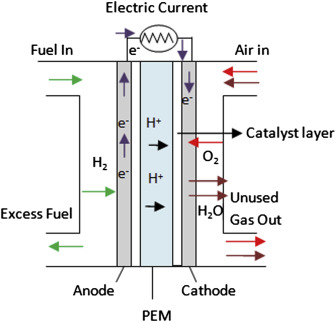
\includegraphics{figures/pemfccell.jpg}
    \caption{Schematic of a PEMFC cell \cite{Dharmalingam2019}}
    \label{fig:pemfccell}
\end{figure}

\begin{equation} \label{pemfcanode}
    H_2 \rightarrow 2H^+ + 2e^-
\end{equation}
\begin{equation} \label{pemfccathode}
    \frac{1}{2}O_2 + 2H^+ + 2e^- \rightarrow H_2 O
\end{equation}
\begin{equation} \label{pemfcall}
    H_2 + \frac{1}{2} \rightarrow H_2O
\end{equation}

While a number of fuel cell technologies can use hydrogen as a fuel source, the most suitable for FCEV's, and in particular mass production of affordable vehicles, are proton exchange membrane fuel cells (PEMFC). This is due to their high power density, low start up time, and low operating temperatures. \cite{Alaswad2016}

A PEMFC uses a proton conducting polymer membrane as an electrolyte material, typically nafion. A PEMFC cell consists of two metal bipolar plates which act to distribute the fuel and oxident within the cell, aid water management within the cell, separate individual cells in a fuel cell stack, and carry current away from the cell. \cite{Alaswad2016} A Membrane electrode assembly (MEA) which consists of the polymer membrane, two dispersed noble metal catalyst layers to enable the anode and cathode reactions, and two gas diffusion layers to ensure uniform access of fuel and oxident to the catalyst layer. Common materials for the MEA are shown in figure \ref{fig:MEA}\cite{Mehta2003}. The components are wedged between two rubber seals to ensure gas the cell is gas tight. Individual cells are combined in series to form a fuel cell stack which can provide the desired power as shown in \ref{fig:pemfcstack}

\begin{figure}[H]
    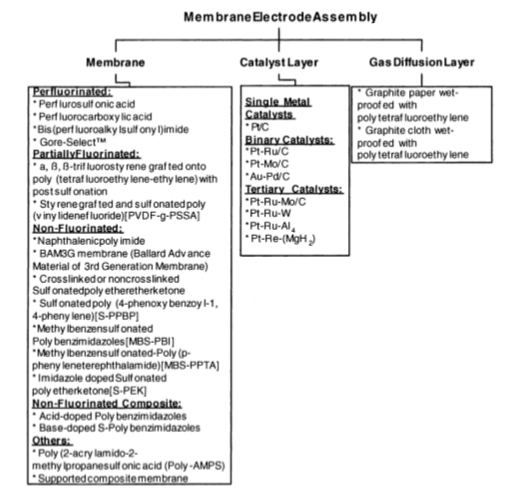
\includegraphics[scale=0.7]{figures/MEA.png}
    \caption{Classification of MEA materials \cite{Mehta2003}}
    \label{fig:MEA}
\end{figure}

\begin{figure}[H]
    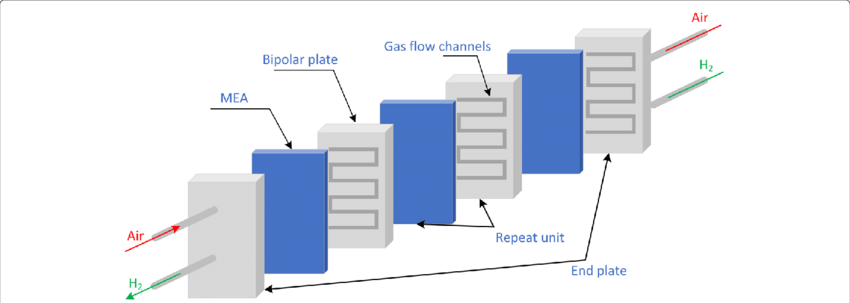
\includegraphics[scale=0.5]{figures/PEMFCstack.png}
    \caption{Schematic of a PEMFC stack \cite{Li2019}}
    \label{fig:pemfcstack}
\end{figure}

\subsection{Hydrogen Production}
Hydrogen production refers to a range of industrial processes for generating hydrogen. 
Since there are no natural reserves of hydrogen, it must be obtained through one of these methods. The most important factor for determining the feasibility of a hydrogen production process is the primary source of energy that is used. Currently the options for this are nuclear energy in the form of heat, renewable energy in the form of heat, electricity, light, or fossil fuels. 
Currently the primary sources of hydrogen are from fossil fuels: steam reforming of methane accounts for 48\% and other hydrocarbons account for 30\% of global hydrogen production; gasification of coal accounts for 18\%; and electrolysis of water accounting for the remaining 4\%. \cite{Mangold2009} Electrolysis and SMR will be discussed since these are expected to be the most dominant production methods in the future. \cite{Holladay2009}

\subsubsection{Hydrogen from fossil fuels and hydrocarbons}
Fossil fuels are the most dominant source of hydrogen production \cite{Mangold2009} and there are a number of processes which are commonly utilized in industry. The most popular and therefore the ones which will be discussed are steam methane reforming and hydrocarbon decomposition.

\paragraph{Steam Methane reforming} is the conventional and most economical method for producing hydrogen, and it has been predicated by the 
IEA that this trend will continue despite the emergence of other hydrogen production methods. \cite{InternationalEnergyAgencyIEA2015}
Steam methane reforming occurs through a two-step chemical process. If another hydrocarbon other than methane is being used it must first be pre-reformed into methane as shown in equation \ref{smr1}. A schematic representation of the process can be seen in figure \ref{fig:smrprocess}

\begin{figure}
    \centering
    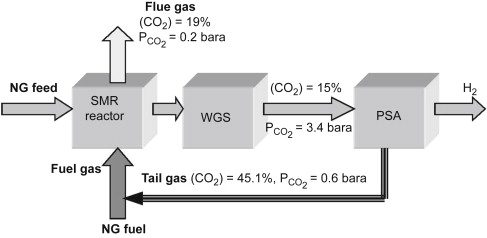
\includegraphics{figures/smrprocess.jpg}
    \caption{Simplified block diagram of a typical modern SMR plant. WGS is a water gas shift reactor. CO\textsubscript{2} concentrations are in mol.\%. \cite{Muradov2015}}
    \label{fig:smrprocess}
\end{figure}

\begin{equation} \label{smr1}
    C_n H_m + H_2 O \rightarrow nCO +(\frac{n+m}{2})H_2 
\end{equation}
\begin{equation}\label{smr2}
    CH_4 + H_2 O \rightarrow CO + 3H_2 \quad \Delta H_{298K}^o = +205 kJ/mol
\end{equation}
\begin{equation}\label{smr3}
    CO+ H_2 O \rightarrow CO_2 + H_2 \quad \Delta H_{298K}^o = -41 kJ/mol
\end{equation}

Equation \ref{smr2} takes place in a reactor operating at 700-850\textdegree C, at pressures of 3-25 bar, and in the presence of a nickel based catalyst. \cite{Muradov2015}
The result of this step is a mixture of CO and H\textsubscript{2}, commonly referred to as syngas. 
This syngas is further used as a feedstock for the reaction shown in equation \ref{smr3} known as water gas 
shift in order to produce greater hydrogen yields.  
This step is carried out in a two-step reaction. An initial high temperature stage at 350\textdegree C which converts majority of the syngas to CO\textsubscript{2} and hydrogen, and a final low-temperature step which operates at 250\textdegree C which utilizes a catalyst with higher activity to minimise the remaining CO\textsubscript{2}. \cite{Muradov2015}
The final product will be a mixture of CO\textsubscript{2} and H\textsubscript{2}.  

A number of separation steps are used in order to prevent impurities from contaminating the 
resulting gas mixture. The traditional separation step is pressure swing adsorption (PSA) which takes 
advantage of adsorption of gaseous molecules onto a molecular sieve at high pressures. Hydrogen purities of \textasciitilde99.9\% are achievable using this method however the cost is high and typically contributes to around 
20-30\% of the total production cost. \cite{Muradov2015} The other main separation step is desulphurization which uses a 
combination of CoMo and ZnO catalysts in series at 450-550\textdegree C to remove sulphur. \cite{Muradov2015}
This step is essential to ensure sulphur is not present in the gas exit stream and also to ensure catalyst 
poisoning does not occur at any point in the process. 

\paragraph{Hydrocarbon decomposition} is a process by which hydrocarbon molecules are converted into solid carbon and hydrogen. \cite{Ahmed2009} This reaction is typically operated either thermally or by creating a plasma. A metallic catalyst such as nickel or iron is required. The reaction is shown in equation \ref{eq:4} \cite{Muradov2008} 

\begin{equation}\label{eq:4}
    C_x H_2x+2 \rightarrow xC + (x+1)H_2
\end{equation}

An advantage of this process is that the only feedstock is the hydrocarbon, so presuming that the feedstock is sufficiently pure this method of hydrogen production should remove the needs for further downstream processing. \cite{Ahmed2009} The main disadvantage of this method is the since solid carbon is the main by-product the catalyst will be easily deactivated and will require regular maintenance to ensure carbon build up is managed. \cite{Ahmed2009}

\subsubsection{Hydrogen from water}

\paragraph{Electrolysis} uses an electric current to split water into hydrogen and oxygen using separate anode and cathode chambers isolated using an ion exchange membrane. The anode and cathode reactions are shown in equations \ref{electrolysis1} and \ref{electrolysis2}. The main competitive advantage of electrolysis is that reactors are modular and highly scalable, allowing hydrogen to be produced in a distributed manner. \cite{Acar2014} The main input to the process is electricity and if this electricity is produced using renewable sources then the process can be considered carbon neutral. However if a non-renewable source of energy is used the net carbon produced per mole of hydrogen would be higher than that produced by SMR. \cite{Koroneos2004}
Electrolysis is incentivised by the increasing price of natural gas and the decreasing price of electricity, which some predict will result in electrolysis becoming more economically feasible than SMR in the future. \cite{Acar2014}

\begin{equation}\label{electrolysis1}
2H_2 O +  2e^- \rightarrow H_2 + 2OH^-
\end{equation}
\begin{equation}\label{electrolysis2}
2OH^- \rightarrow \frac{1}{2}O_2+ H_2 O + 2e^-
\end{equation}

\paragraph{Thermal decomposition of water} is the process of splitting water into hydrogen and oxygen at temperatures of 2000\textdegree C as shown in equation \ref{thermdec}. \cite{Holladay2009} The operating temperature of the reaction can be lowered under the presence of a nickel or iron based catalyst. \cite{Holladay2009} Due to the high energy demand for this production method water splitting is not a feasible method of commercial hydrogen production.

\begin{equation}\label{thermdec}
    H_2 O \rightarrow H_2 + \frac{1}{2} O_2  \quad \Delta H_{298K}^o = +286 kJ/mol
\end{equation}

\subsection{Hydrogen impurities in the supply chain}
The method used to manufacture hydrogen will affect which potential impurities can be present in the final product. While steps are taken in both electrolysis and SMR to ensure a pure product is produced, there is still the chance of impurities reaching the customers fuel cell. This section will explore how ISO 14687-2 impurities can enter the supply chain, and their effect on the operation of a PEMFC. A summary is shown in table \ref{impuritytbl}
\begin{table}[]
    \caption{Summary of ISO 14687-2 impurities in the supply chain and their effects on fuel cell operation adapted from \cite{Bacquart2018}}
    \resizebox{\textwidth}{!}{\begin{tabular}{@{}ccccc@{}}
    \toprule
    Impurity                               & Production sources & Contamination source                                                                                                                                                                     & Contamination barriers                                                                                                                                                            & Effect on fuel cell operation                                                                                                                                       \\ \midrule
    \multirow{2}{*}{N\textsubscript{2}}                    & SMR                & \begin{tabular}[c]{@{}c@{}}Raw material\\ PSA malfunction\end{tabular}                                                                                                                   & PSA                                                                                                                                                                               & \multirow{4}{*}{Reduced energy density of fuel}                                                                                                                     \\
                                           & Electrolysis       & \begin{tabular}[c]{@{}c@{}}Maintenance\\ Leakage\\ Air intake into water tank\end{tabular}                                                                                & \begin{tabular}[c]{@{}c@{}}Maintainance\\ PEM membrane\\ H\textsubscript{2} pressure \textgreater N\textsubscript{2} pressure supply\end{tabular}              &                                                                                                                                                                     \\
    Ar                                     & SMR                & Raw materials                                                                                                                                                                            & PSA                                                                                                                                                                               &                                                                                                                                                                     \\
    He                                     & -                  & -                                                                                                                                                                                        & -                                                                                                                                                                                 &                                                                                                                                                                     \\
    O\textsubscript{2}                                     & Electrolysis       & \begin{tabular}[c]{@{}c@{}}Generation at the anode\\ Membrane cross over\\ TSA malfunction\end{tabular}                                                              & \begin{tabular}[c]{@{}c@{}}TSA operating condition\\ Oxygen sensor\end{tabular}                                                                                                   & \begin{tabular}[c]{@{}c@{}}Potential damage to hydrogen storage\end{tabular} \\
    CO                                     & SMR                & \begin{tabular}[c]{@{}c@{}}By-product\\ Raw materials\end{tabular}                                                                                                                       & \begin{tabular}[c]{@{}c@{}}PSA\\ CO sensor on line\end{tabular}                                                                                                                   & Temporary electrocatalyst poisoning                                                                                                                                 \\
    \multirow{2}{*}{CO\textsubscript{2}}                   & SMR                & \begin{tabular}[c]{@{}c@{}}By-product\\ Raw materials\end{tabular}                                                                                                                       & PSA                                                                                                                                                                               & \multirow{2}{*}{\begin{tabular}[c]{@{}c@{}}Damage to hydrogen storage medium\\ Could cause formation of CO\end{tabular}}                                  \\
                                           & Electrolysis       & \begin{tabular}[c]{@{}c@{}}Water at anodic side\\ Air into the pure water tank\end{tabular}                                                                                              & \begin{tabular}[c]{@{}c@{}}CO\textsubscript{2} filter\\ Anodic separator tank\\ Ion exchange resin \\in closed water loop\\ PEM membrane\end{tabular} &                                                                                                                                                                     \\
    CH\textsubscript{4}                                    & SMR                & Raw material                                                                                                                                                                             & \begin{tabular}[c]{@{}c@{}}PSA\\ Methane sensor on line\end{tabular}                                                                                                              & Reduced energy density of fuel                                                                                                                                      \\
    \multirow{2}{*}{H\textsubscript{2}O}                   & SMR                & Raw material                                                                                                                                                                             & PSA                                                                                                                                                                               & \multirow{2}{*}{\begin{tabular}[c]{@{}c@{}}Ice formation during refilling\\ K+ and Na+ contamination \\ reducing cathode side conductivity\end{tabular}}            \\
                                           & Electrolysis       & \begin{tabular}[c]{@{}c@{}}Reactant\\ Through PEM membrane\\ Hydrogen output water saturated\\ TSA malfunction\end{tabular}                                                              & \begin{tabular}[c]{@{}c@{}}TSA dryer\\ Dew point monitor\\ Operating procedure\end{tabular}                                                                                       &                                                                                                                                                                     \\
    Total sulphur compounds                & SMR                & Raw material                                                                                                                                                                             & \begin{tabular}[c]{@{}c@{}}Desulfuration unit\\ Sulphur trap in reforming system \\ PSA\\ Stainless steel pipe and vessl\end{tabular}                & Permanent electrocatalyst poisoning                                                                                                                                 \\
    \multirow{2}{*}{NH\textsubscript{3}}                   & SMR                & Raw material                                                                                                                                                                             & PSA                                                                                                                                                                               & \multirow{2}{*}{Reduced ion exchange capacity}                                                                                                          \\
                                           & Electrolysis       & Water at anodic side                                                                                                                                                                     & \begin{tabular}[c]{@{}c@{}}Reverse osmosis \\ PEM membrane\end{tabular}                                                                                          &                                                                                                                                                                     \\
    Formaldehyde                           & SMR                & Raw material                                                                                                                                                                             & PSA                                                                                                                                                                               & Temporary electrocatalyst poisoning                                                                                                                                 \\
    Formic acid                            & SMR                & Raw material                                                                                                                                                                             & PSA                                                                                                                                                                               & Temporary electrocatalyst poisoning                                                                                                                                 \\
    \multirow{2}{*}{Halogenated compounds} & SMR                & Raw material                                                                                                                                                                             & \begin{tabular}[c]{@{}c@{}}Desulfuration unit\\ Chlorinated trap in reforming system \\ PSA\\ Stainless steel pipe and vessel\end{tabular}           & \multirow{2}{*}{Permanent electrocatalyst poisoning}                                                                                                                \\
                                           & Electrolysis       & \begin{tabular}[c]{@{}c@{}}Raw material contamination\end{tabular} & Reverse osmosis\\Monitoring Cl\textsubscript{2} concentration                                                                                                                                      &                                                                                                                                                                     \\ \bottomrule
    \end{tabular}}\label{impuritytbl}
    \end{table}

    
\subsubsection*{Water}
Water can be present from both SMR and electrolysis due to it being a main by-product of SMR reactions, and the main reactant in electrolysis. 

The PSA process used in SMR is an appropriate barrier to prevent water contaminating the end product. This is due to the molecular sieves commonly used  having a high selectivity for water. \cite{Muradov2015} When a PSA system is designed to produce an output of CO below 0.2 \textmu mol/mol, the concentration of water will be less than 0.1 \textmu mol/mol. \cite{Bacquart2018} This makes it unlikely for H\textsubscript{2}O to be present in hydrogen produced using this method.

There are three potential pathways for water to contaminate hydrogen through electrolysis. These are:
\begin{itemize}
    \item Electro-osmosis through the proton exchange membrane
    \item Hydrogen water saturated at 60\textdegree C
    \item Drier malfunction
\end{itemize}
Modern electrolysers are fitted with a drier, which is the main barrier for water vapour exiting the process with hydrogen. \cite{Bacquart2018} In the event of drier failure, most systems are fit with a dew point analyser that will trip, shutting off production until the issue can be fixed. \cite{Bacquart2018}

Water generally does not affect the function of a fuel cell, however; it provides a transport mechanism for water-soluble contaminants such as K+ and Na+ \cite{InternationalStandardISO14687-2:20122012} to pass through the electrolyte and have a negative long-term effect on the conductivity of the cathode side of the membrane. In addition, water may increase the risk of ice formation within vehicle fuel storage and hydrogen dispensing systems under certain conditions. 

\subsubsection*{Total hydrocarbon content}
The presence of hydrocarbons are most likely to result from the SMR process. Hydrocarbons are not expected to be present at all in electrolysis. Similar to water contamination through SMR, the most likely reason for hydrocarbon contamination is due to malfunction of the PSA system used to purify the product hydrogen. 

A PSA system designed to deliver hydrogen with a CO concentration <0.2 \textmu mol/mol should be sufficient to reduce the amount fraction of hydrocarbons to below the 5 \textmu mol/mol required by ISO 14687. \cite{Bacquart2018}

Different hydrocarbons have different effects on fuel cell performance. Generally aromatic hydrocarbons adsorb more strongly on the catalyst surface than other hydrocarbons, inhibiting access to hydrogen.\cite{InternationalStandardISO14687-2:20122012} Methane (CH\textsubscript{4}) is generally considered an inert constituent and it's main effect on fuel cell performance is  diluting the hydrogen fuel stream. \cite{InternationalStandardISO14687-2:20122012}

\subsubsection*{Oxygen}
In SMR processes oxygen is not used as a raw material, nor is it stable during the process conditions, readily reacting with hydrogen to produce water. In addition to this the oxygen content of the feedstock to the PSA separation stage must be below a certain level for safety reasons. Therefore oxygen contamination from hydrogen produced from SMR is unlikely. 

Oxygen is a main by-product of electrolysis, although is generated at the anode side of the electrolysis stack. Likely methods of contamination are through cross over through the PEM membrane. Due to the danger of high oxygen levels in hydrogen streams, most electrolysis systems are fit with an oxygen sensor that trips the system if the concentration of oxygen in the hydrogen stream surpasses 5 umol/mol. \cite{Bacquart2018}

Oxygen in low concentrations does not adversely affect the function of the fuel cell system; however, it may be a concern for some on-board vehicle storage systems, for example, by reaction with metal hydride storage materials. \cite{InternationalStandardISO14687-2:20122012} 

\subsubsection*{Helium, nitrogen and argon}
Helium is not present as a feed material in any of the discussed processes, however there is also no barrier to Helium in the exit stream and therefore any helium that enters a SMR or electrolysis process will not be removed. Despite this it is unlikely that helium will be present in a hydrocarbon feedstock, or water.

Argon is similar to helium, however it is more likely for Argon to be present in the natural gas feedstock for SMR. Unlike helium, the PSA step in SMR can act as a barrier for Argon, however this will depend on the specific molecular sieve used in the system. \cite{Bacquart2018}

Nitrogen is the most likely inert impurity to be present in fuel cell hydrogen, this is due to the abundance of nitrogen in the air which the system could be exposed to, and the frequency at which nitrogen is used as a functional gas in processes for purging chambers, actuating valves etc.

Inert constituents, such as helium (He), nitrogen (N\textsubscript{2}) and argon (Ar) do not adversely affect the function of fuel cell components or a fuel cell system. However, they dilute the hydrogen gas. N\textsubscript{2} and Ar especially can affect system operation and efficiency and can also affect the accuracy of mass metering instruments used for hydrogen dispensing. \cite{InternationalStandardISO14687-2:20122012}

\subsubsection*{Carbon dioxide} 
Like most other impurities which are present in SMR, CO\textsubscript{2} is likely to be removed from the SMR process at the PSA step, with most commonly used molecular sieves being able to remove carbon dioxide during normal operation. \cite{Muradov2015} 

CO\textsubscript{2} can be present in the water used for electrolysis although there are several interlocks to prevent it reaching the exit stream. Most electrolysis systems have a CO\textsubscript{2} filter on the inlet and a reverse osmosis unit to ensure the purity of the inlet water. An anodic separation tank which features an ion exchange resin in a closed water loop also acts as an additional barrier, and finally CO\textsubscript{2} has a low crossover potential through the PEM membrane and therefore is unlikely to cross into the cathode side of the system.\cite{Bacquart2018}

CO\textsubscript{2} does not typically affect the function of fuel cells. However, CO\textsubscript{2} may adversely effect on board hydrogen storage systems using metal hydride alloys. With CO\textsubscript{2}, at levels higher than the specification, a reverse water gas shift reaction can occur under certain conditions in fuel cell systems to create carbon monoxide. \cite{InternationalStandardISO14687-2:20122012}


\subsubsection*{Carbon monoxide}
Carbon monoxide is a main byproduct of SMR which is separated from the exit gas stream through PSA. \cite{Muradov2015} If this fails SMR processes are fitted with a CO sensor to ensure the concentration in the product does not pass a certain threashold. \cite{Bacquart2018} It is unlikely for CO to be present from electrolysis.

Carbon monoxide (CO) is a severe catalyst poison that adversely effects fuel cell performance by inducing a competitive adsorption effect between itself and hydrogen on the electrocatalyst surface. The result is a temporary reduction in operating efficiency. \cite{InternationalStandardISO14687-2:20122012} Although its effect can be reversed through mitigating strategies, such as material selection of membrane electrode assembly (MEA), system design, and operating conditions, it's effect on operation is still a concern. Lower catalyst loadings are particularly susceptible to catalyst poisoning contaminants.

\subsubsection*{Total sulfur compounds}
Sulphur contamination is most likely to come from hydrogen produced from hydrocarbon sources. 
Since the SMR process also uses catalysts that are susceptible to poisoning from sulphur compounds all plants are fit with a desulphurisation unit upstream from the main process. \cite{Muradov2015} This is designed to reduce the concentration of sulphurous compounds to <50 nmol/mol. \cite{Bacquart2018}

Should the desulphurisation unit fail the catalysts used in both reforming steps will be deactivated, preventing the process from operating and will likely result in shut down of the plant. PSA also acts as a final barrier, since H\textsubscript{2}S will adsorb onto the molecular sieves more strongly than CO. \cite{Bacquart2018}

The other potential source of sulphur contamination is the potential release from any gasket materials used in the process. This can be easily prevented by ensuring only materials that do not contain sulphur are used. \cite{InternationalStandardISO14687-2:20122012}. It is unlikely that sulphur contamination will arise from electrolysis. 

Sulfur containing compounds are severe catalyst poisons that at even very low levels can cause irreversible degradation of fuel cell performance due to a permanant reaction taking place between sulphur and the platinum catalyst. The specific sulfur compounds addressed in particular are: hydrogen sulfide (H\textsubscript{2}S), carbonyl sulfide (COS), carbon disulfide(CS\textsubscript{2}), methyl mercaptan (CH\textsubscript{3}SH). \cite{InternationalStandardISO14687-2:20122012} 

\subsubsection*{Formaldehyde and formic acid}
Formaldehyde (HCHO) and formic acid (HCOOH) is a produced through a side reaction in SMR depending on the specific operating conditions of the process.\cite{Muradov2015} PSA is the main barrier for preventing contamination of the product. \cite{Bacquart2018}

Formaldehyde and formic acid have a similar effect on fuel cell performance as CO and are thus considered as reversible contaminants. The effect of HCHO and HCOOH on fuel cell performance can be more severe than that of CO due to slower recovery kinetics and their specifications are lower than that for CO. \cite{InternationalStandardISO14687-2:20122012} Lower catalyst loadings are particularly susceptible to catalyst poisoning contaminants.

\subsubsection*{Ammonia}
Hydrogen could be contaminated with ammonia through either SMR or electrolysis. Ammonia is a by-product of the reforming steps and PSA should be sufficient to remove ammoinia from the exit stream of SMR. Ammonia can also be present in water used in electrolysis however the reverse osmosis step used to purify the water before the process is normally sufficient in removing all ammonia before it is used in the process. \cite{Bacquart2018}

Ammonia (NH\textsubscript{3}) causes some irreversible fuel cell performance degradation by affecting the ion exchange capacity of the ionomer of the proton exchange membrane. \cite{InternationalStandardISO14687-2:20122012}

\subsubsection*{Total halogenated compounds} 
Halogenated compounds can contaminate hydrogen by entering either SMR or electrolysis through the process input, or leaking into the process at other points where they are used. Potential sources include chlor-alkali production processes, refrigerants used in processing, and cleaning agents. \cite{Bacquart2018}

Halogenated compounds cause irreversible performance degradation similar to sulphur, reacting with the platinum electrocatalysts to form platinum-halides such as PtCl\textsubscript{4}. \cite{Dona2009} However the concentrations required to cause this damage has not been well documented in literature.

\section{Research Objectives}
This thesis will focus on developing hydrogen impurity enrichment as a low-cost technique for measuring 
the impurities in fuel grade hydrogen to ISO 14687-2 specification. 
This study will revolve around the membrane materials used to concentrate the impurities in hydrogen samples 
and will aim to determine the best material, and conditions for the hydrogen impurity enrichment device. 
The thesis aims are as follows:
\begin{itemize}
\item Identify the best material for enriching impurities based on the degree of interaction and reactivity with the impurities shown in Table 1 
\item Finalise a protocol for national measurement institutions to follow when enriching a hydrogen sample. 
\item Convert the experimental set up in to a commercially viable prototype which could be used in analytical laboratories
\item Perform full enrichment using these three conclusions on a real sample taken from a hydrogen refuelling station
\end{itemize}
In order to determine suitable enrichment material ‘Density Functional Theory (DFT) will be used to screen a number of materials for their suitability as an impurity enrichment membrane on their simulated 
interaction strength with ISO 14687 impurities. 

The best performing membrane materials simulated in Chapter 3 will then be synthesised in Chapter 4. 
The hydrogen permeability of each material under a number of ISO 14687-2 impurities will be measured to 
validate the simulation results and further narrow down the most suitable membrane composition. 
Following from this the best membrane will be used in Chapter 5 which will describe the design and 
commercialisation of the final hydrogen impurity enrichment device. The design of the enrichment device 
will include an uncertainty budget of the technique, automation of the device, and compliance to European standards.

Finally the new device, featuring the most suitable membrane, redesigned process, and protocols for tracer enrichment will be tested using a real sample taken from a hydrogen refuelling station.

\section{Thesis structure and presentation}
This thesis consists of 7 chapters, which includes the ‘Introduction’, ‘Literature Review’, 
experimental chapters and ‘Conclusion’. The thesis structure is visualised in figure \ref{funnel}. 
The experimental chapters address different aspects of development of hydrogen metrology techniques as 
described above. 

\begin{figure}[H]
  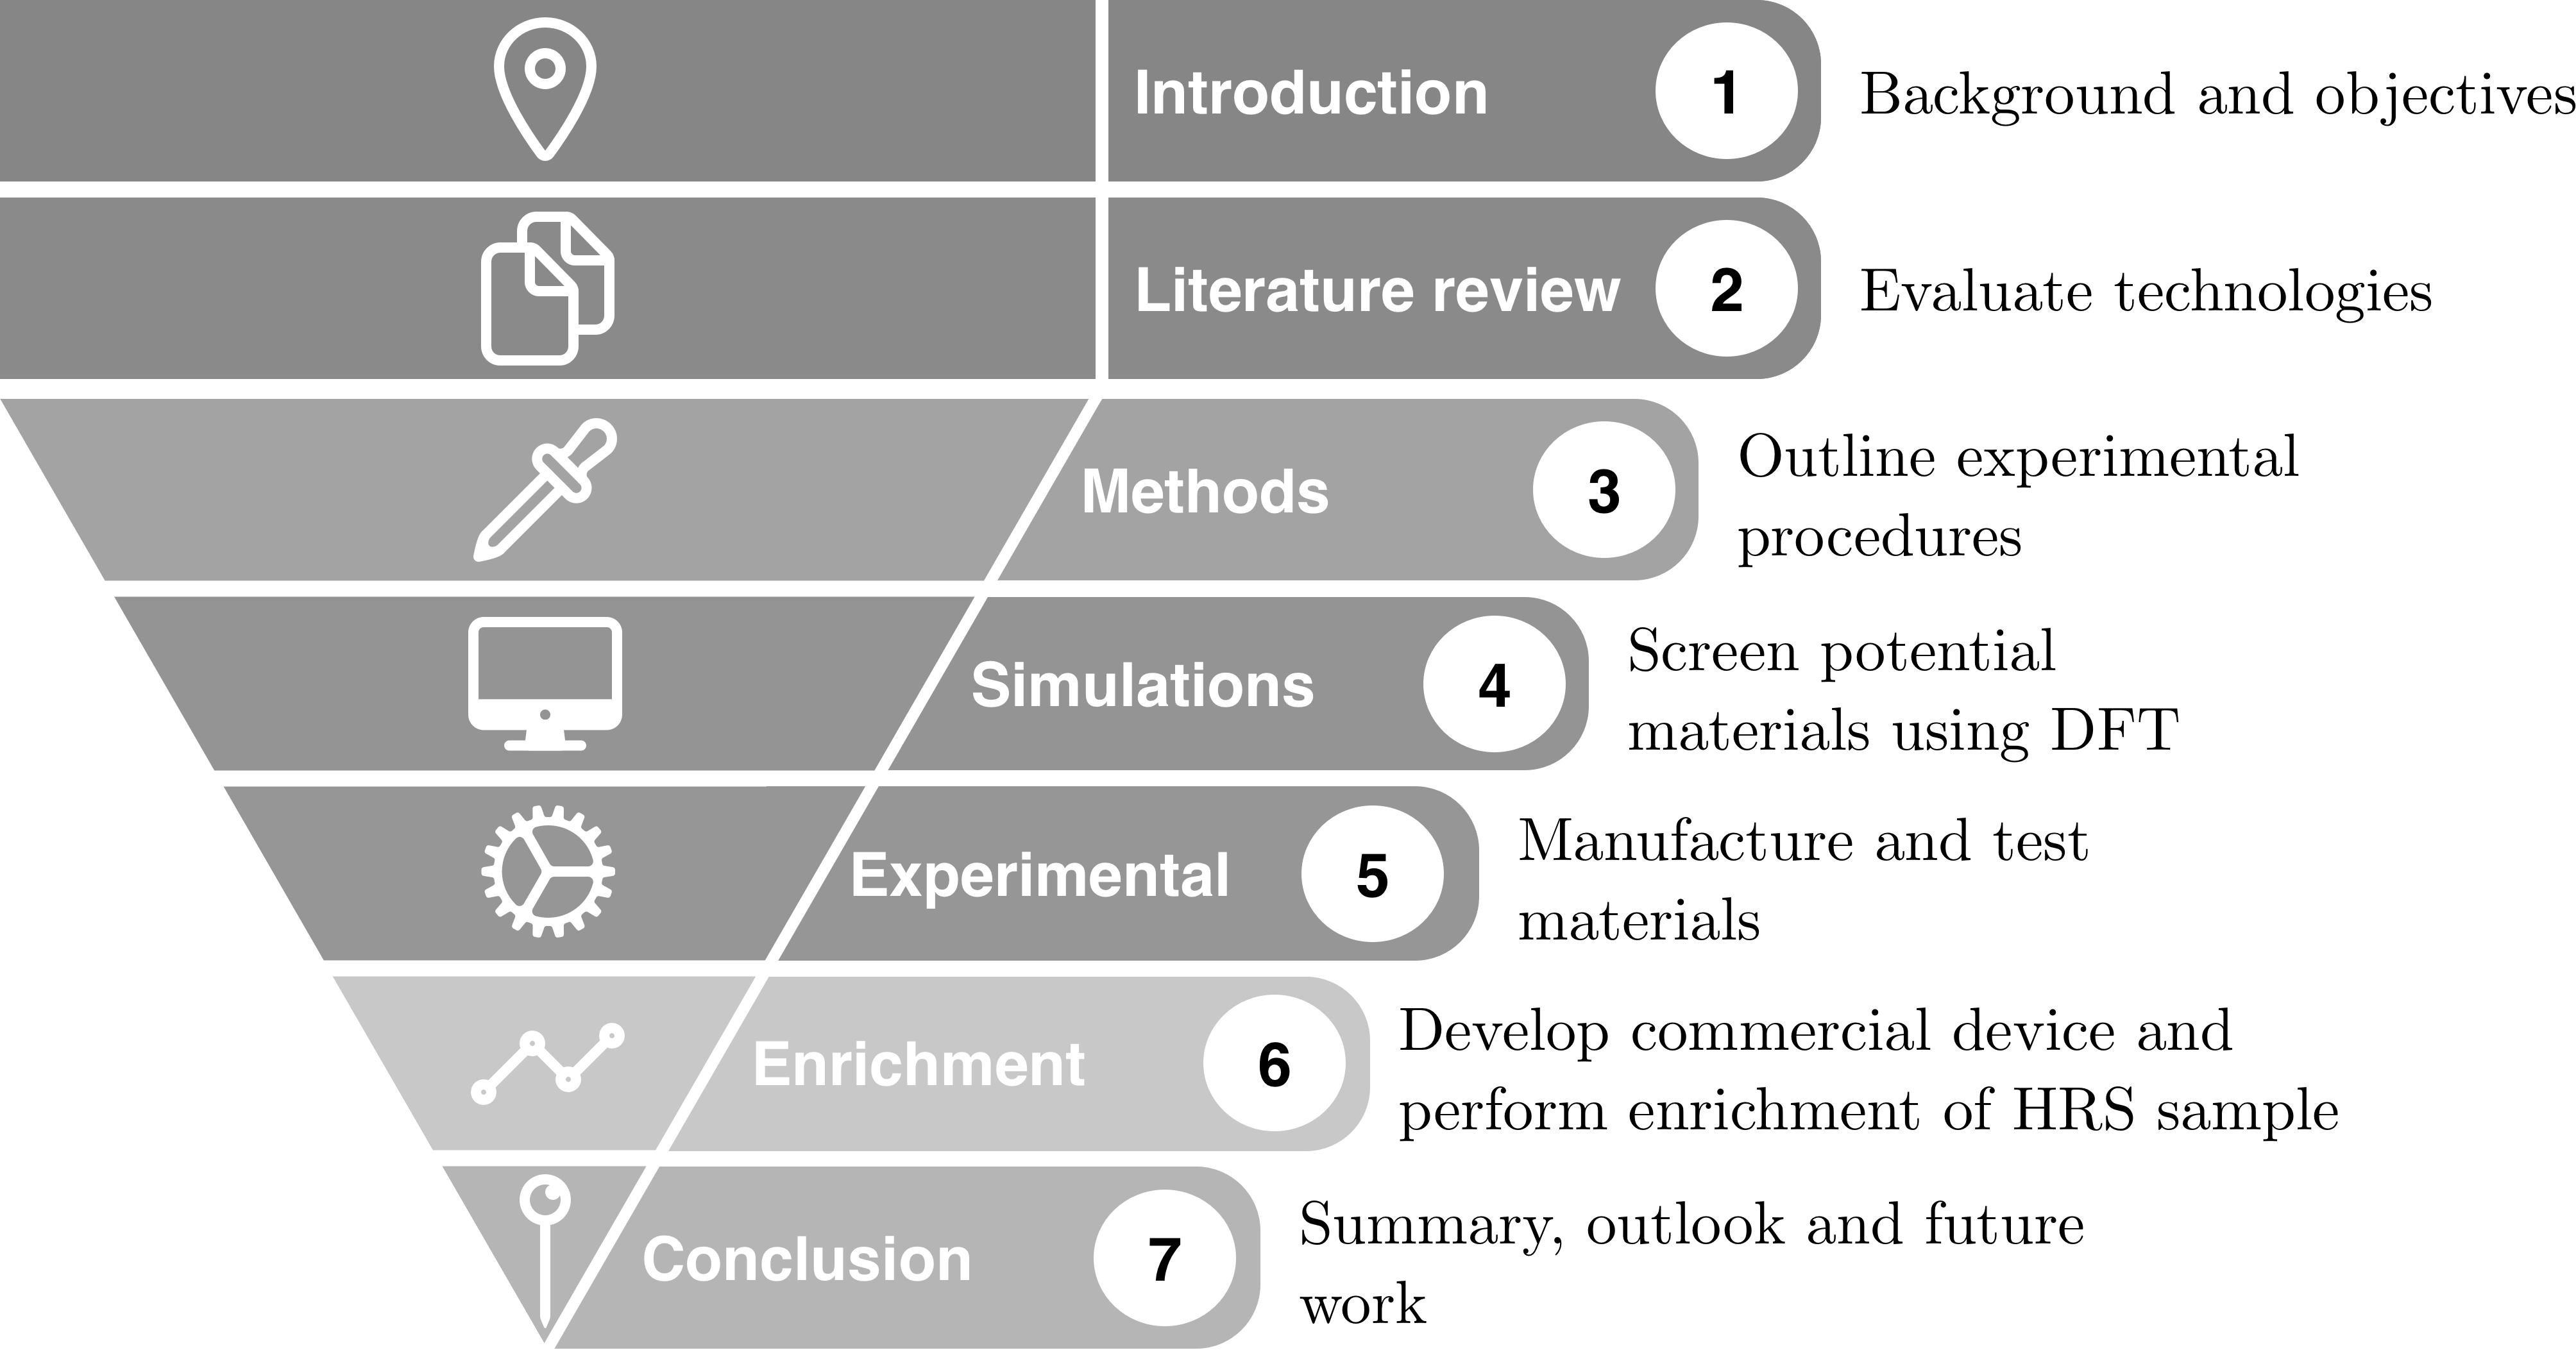
\includegraphics[width=\linewidth]{figures/funnel.png}
  \caption{Schematic presentation of the thesis structure}
  \label{funnel}
\end{figure}


\renewcommand{\bibname}{References}
\bibliographystyle{unsrtnat}
\bibliography{library.bib}